\setchapterpreamble[u]{\margintoc}
\chapter*{Introducción}
\labch{introduction_spanish}
\label{sec:introduction_spanish}

\lettrine[findent=0pt, lines=3]{\textbf{L}}{ }a teledetección ayuda a controlar, predecir y optimizar las actividades de las que dependen procesos del mundo real, y por tanto, a actuar en función de los datos analizados. Existen numerosos sensores que posibilitan esta tarea, los cuales pueden clasificarse en función de la distancia a la que operan, el intervalo de longitudes de onda al que son sensibles y el mecanismo de adquisición de datos, ya sea pasivo o activo. Las dos últimas categorías dependen del mecanismo del dispositivo, mientras que seleccionar una distancia u otra en la adquisición de datos está muy influenciado por el caso de estudio y los objetivos que se persiguen. No obstante, otros factores igualmente relevantes son el presupuesto del que se dispone, así como restricciones de tamaño del sensor, o las propias condiciones ambientales del área de interés. Es posible utilizar sensores que requieren de contacto directo con la superficie que debe monitorizarse para medir variables como humedad, temperatura o cantidad de lluvia. Sin embargo, este tipo de dispositivos necesitan mucho más mantenimiento y son más propensos a deteriorarse en condiciones ambientales adversas \cite{silva_low-cost_2019, morais_versatile_2021}. Además, cada uno de estos sensores envía información de una posición espacial muy específica, que ocupa un lugar en una red lógica de sensores. Por tanto, lo que se hace es discretizar el espacio mediante un conjunto de dispositivos ubicados en forma de malla o en posiciones de especial interés. Por tanto, es difícil trasladar un sistema así para zonas de grandes dimensiones. Además, la disposición de estos sensores, tanto a nivel lógico como físico, debe ser cuidadosamente diseñada para permitir la intra y extra-comunicación utilizando redes y dispositivos que pueden tener un rango y unas capacidades muy limitadas. Por lo tanto, este tipo de monitorización se adapta mejor a aplicaciones que requieren un control constante, eficiente y en tiempo real del área de estudio. 

\marginnote[.1cm]{Las técnicas de \textbf{teledetección} evitan algunas de las limitaciones espaciales que encontramos en otros dispositivos que necesitan contacto directo con la superficie objetivo o la atmósfera. } 
La \textbf{teledetección} ayuda a mitigar algunas de las anteriores desventajas, de tal manera que permite cubrir áreas de grandes dimensiones utilizando plataformas aéreas, plataformas terrestres o satélites. Además, las mediciones se obtiene desde una distancia variable desde la cual se observa y se adquieren datos. La teledetección se define como el arte y la ciencia de adquirir información de objetos y fenómenos sin estar en contacto directo con éstos \cite{lillesand_remote_2015}. El proceso es muy similar al seguido por el ojo humano; los datos se obtienen mediante impulsos generados por estímulos de luz, los cuales a su vez se corresponden con unas longitudes de onda muy específicas. Al menos dos componentes se encuentran involucrados en este proceso de lectura, tanto los sensores como las plataformas en las que éstos se acoplan. Los sensores serán el eje motivador de esta tesis, mientras que las plataformas pueden ser muy variadas. No obstante, inicialmente éstas se limitaban a satélites. 

Por tanto, \textbf{las imágenes de satélite} son más adecuadas para monitorizar cambios a larga escala, utilizando series temporales que abarcan meses, años e incluso décadas. Estos datos permiten comprender la dinámica existente entre el ser humano y la naturaleza, así como el impacto de los fenómenos naturales (Figura \ref{fig:la_palma_landsat8_spanish}). Algunas aplicaciones de dichos conjuntos de datos son el control de uso del suelo, deforestación, cambios en la superficie terrestre y asentamientos urbanos \cite{asokan_change_2019}. No obstante, la resolución espacial y el periodo para revisitar un mismo punto en satélites no comerciales dificulta su aplicabilidad a tareas de monitorización que requieren de un nivel de detalle elevado (Level of detail: \acrshort{lod}). Este nivel de detalle puede referirse tanto la \textbf{resolución espacial} como a la \textbf{resolución temporal}, o a ambas, siendo éstas las principales \textbf{limitaciones} de las imágenes de satélite, además de su elevado coste. A pesar de ello, el uso de imágenes satélite se encuentra en aumento, como muestra la Figura \ref{fig:scopus_search_platforms_spanish}, debido a la cada vez menor distancia representada en un píxel (Ground Sampling Distance: \acrshort{gsd}) así como a la disminución del periodo empleado para revisitar un mismo punto. 
\begin{marginfigure}[-6cm]
	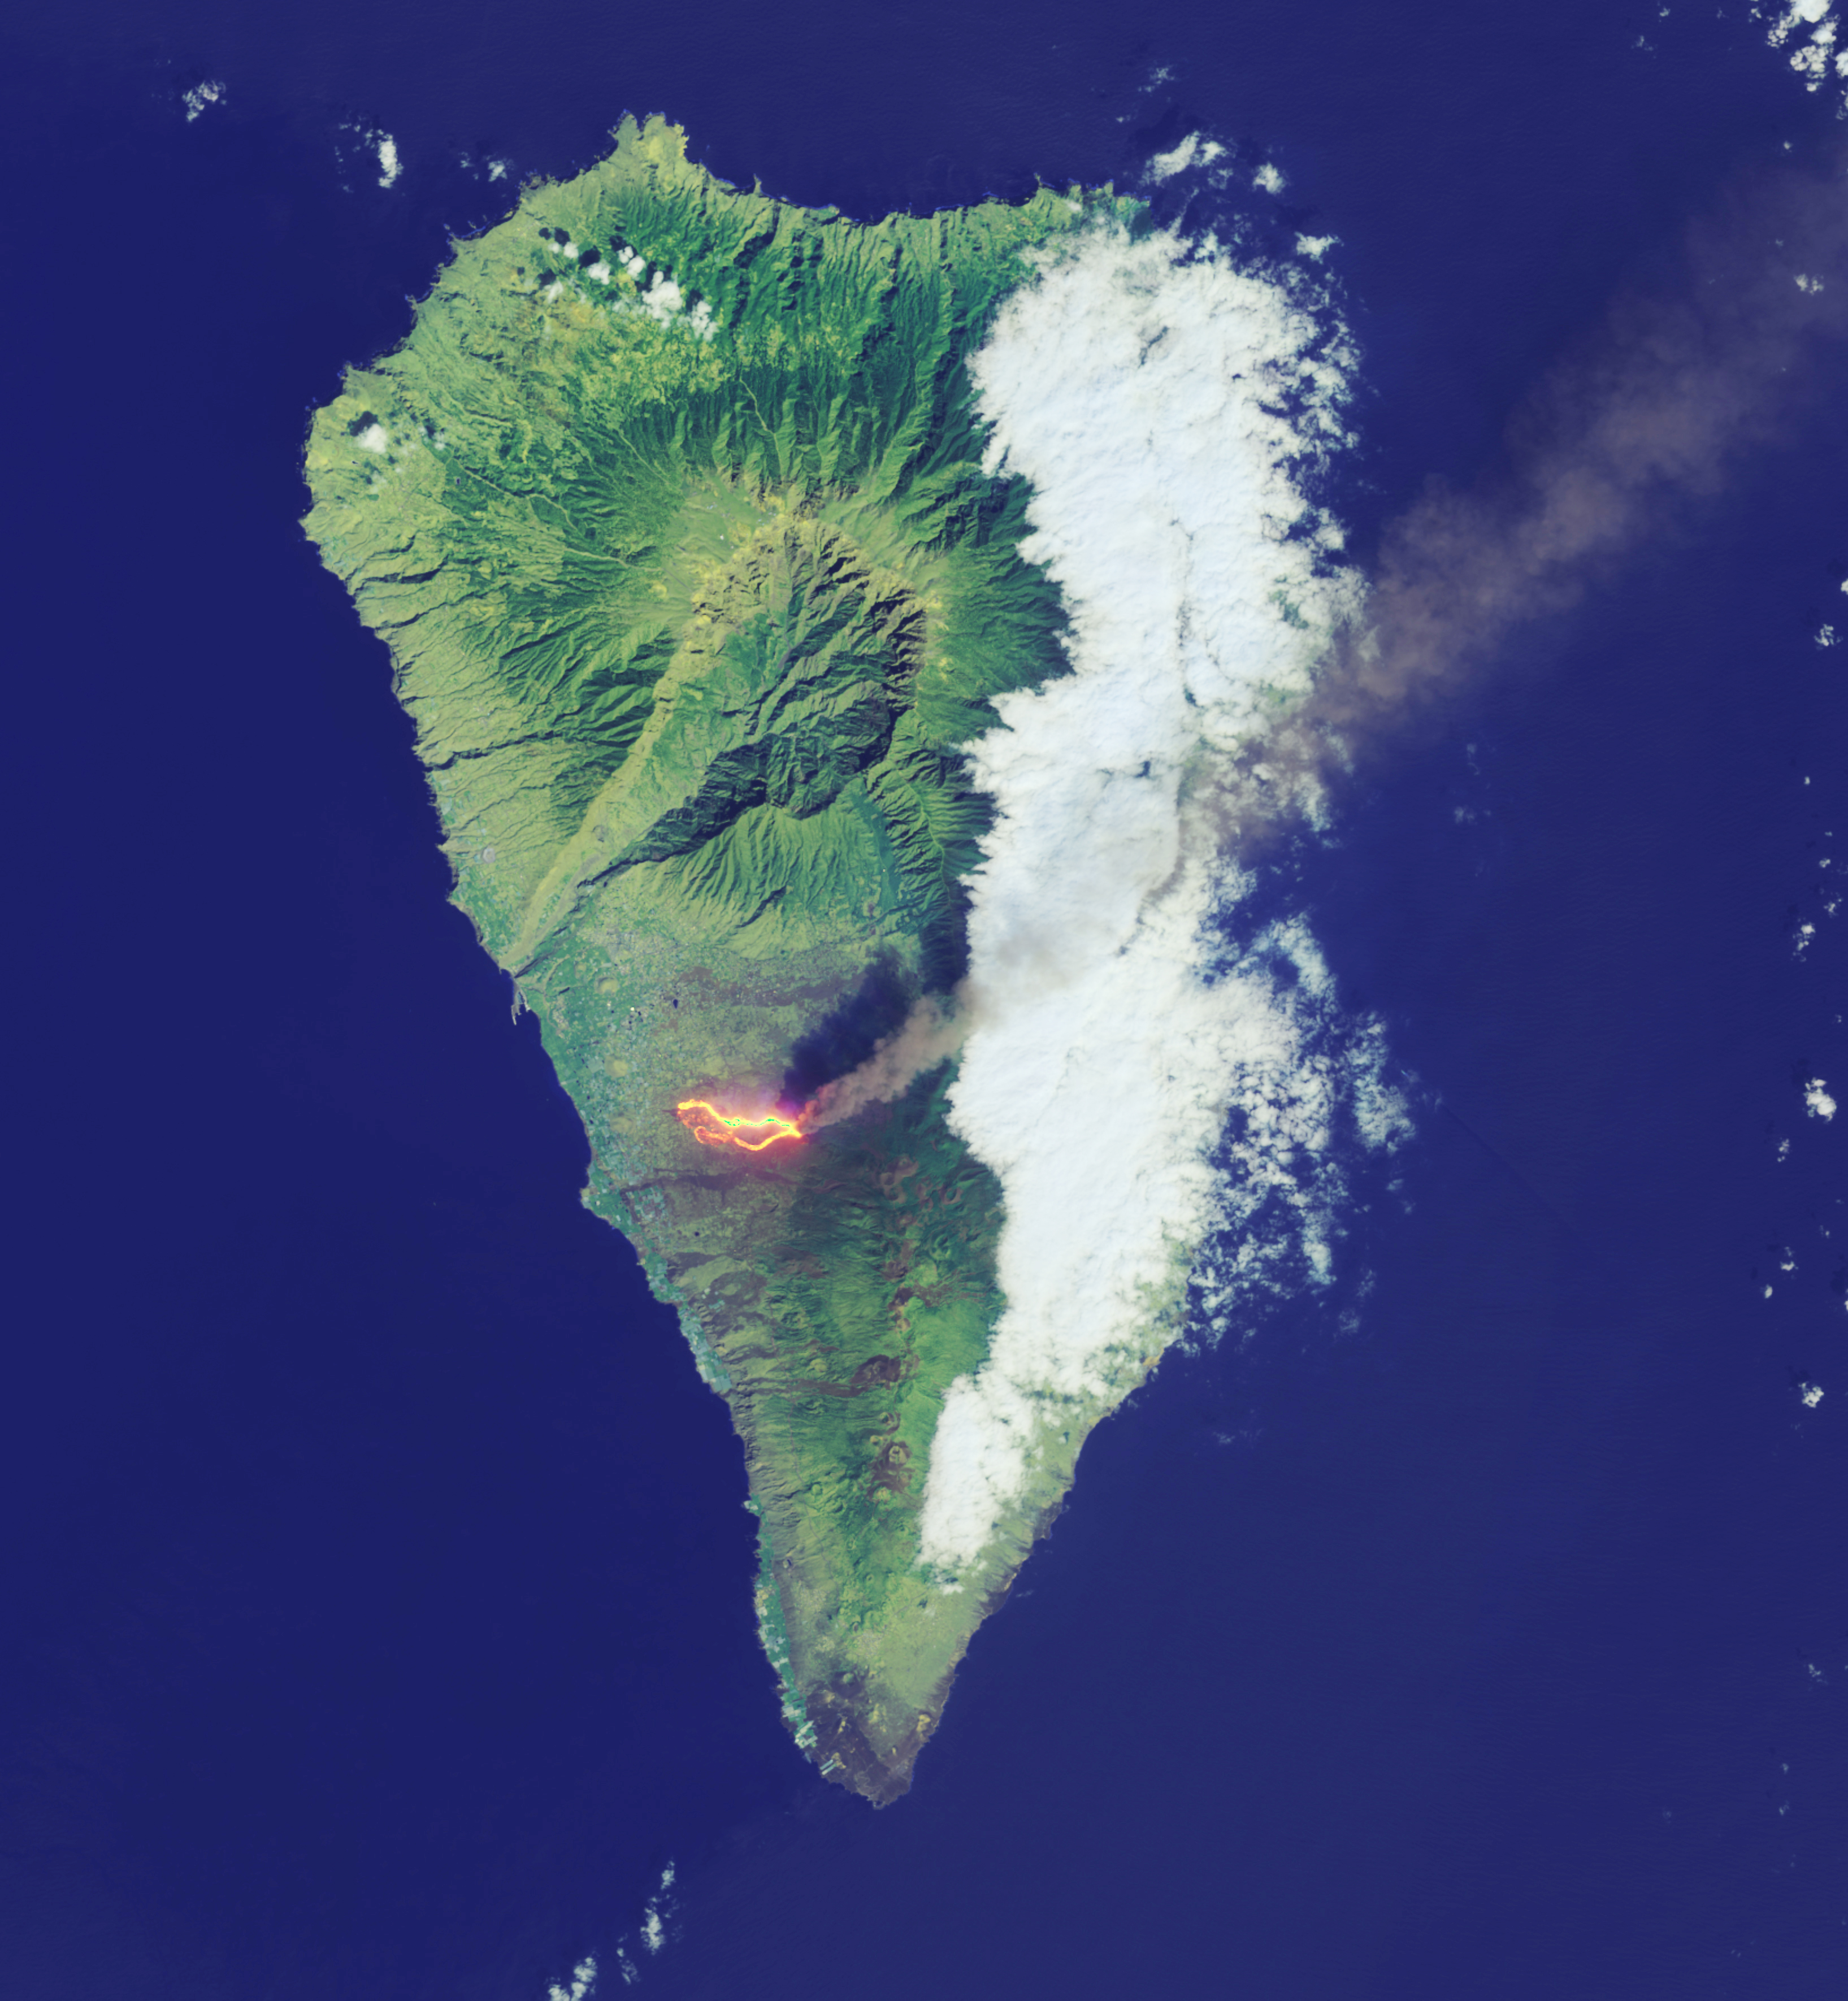
\includegraphics{figs/introduction/landsat8_lapalma.jpg}
	\caption{Cumbre Vieja volcano eruption observed from Landsat-8 \cite{nasa_earth_observatory_lava_2021}.}
	\label{fig:la_palma_landsat8_spanish}
\end{marginfigure}

La Figura \ref{fig:scopus_search_platforms_spanish} muestra el número de artículos que emplean cada una de las plataformas que veremos en este capítulo. La búsqueda realizada en Scopus es la siguiente: $(p_1 \lor p_2 ... \lor p_n) \land (\textit{remote} \hspace{1mm} \land \hspace{1mm} \textit{sensing})$, donde $p_i$ es una de las plataformas que se muestra en la leyenda.

\begin{figure}[!ht]
	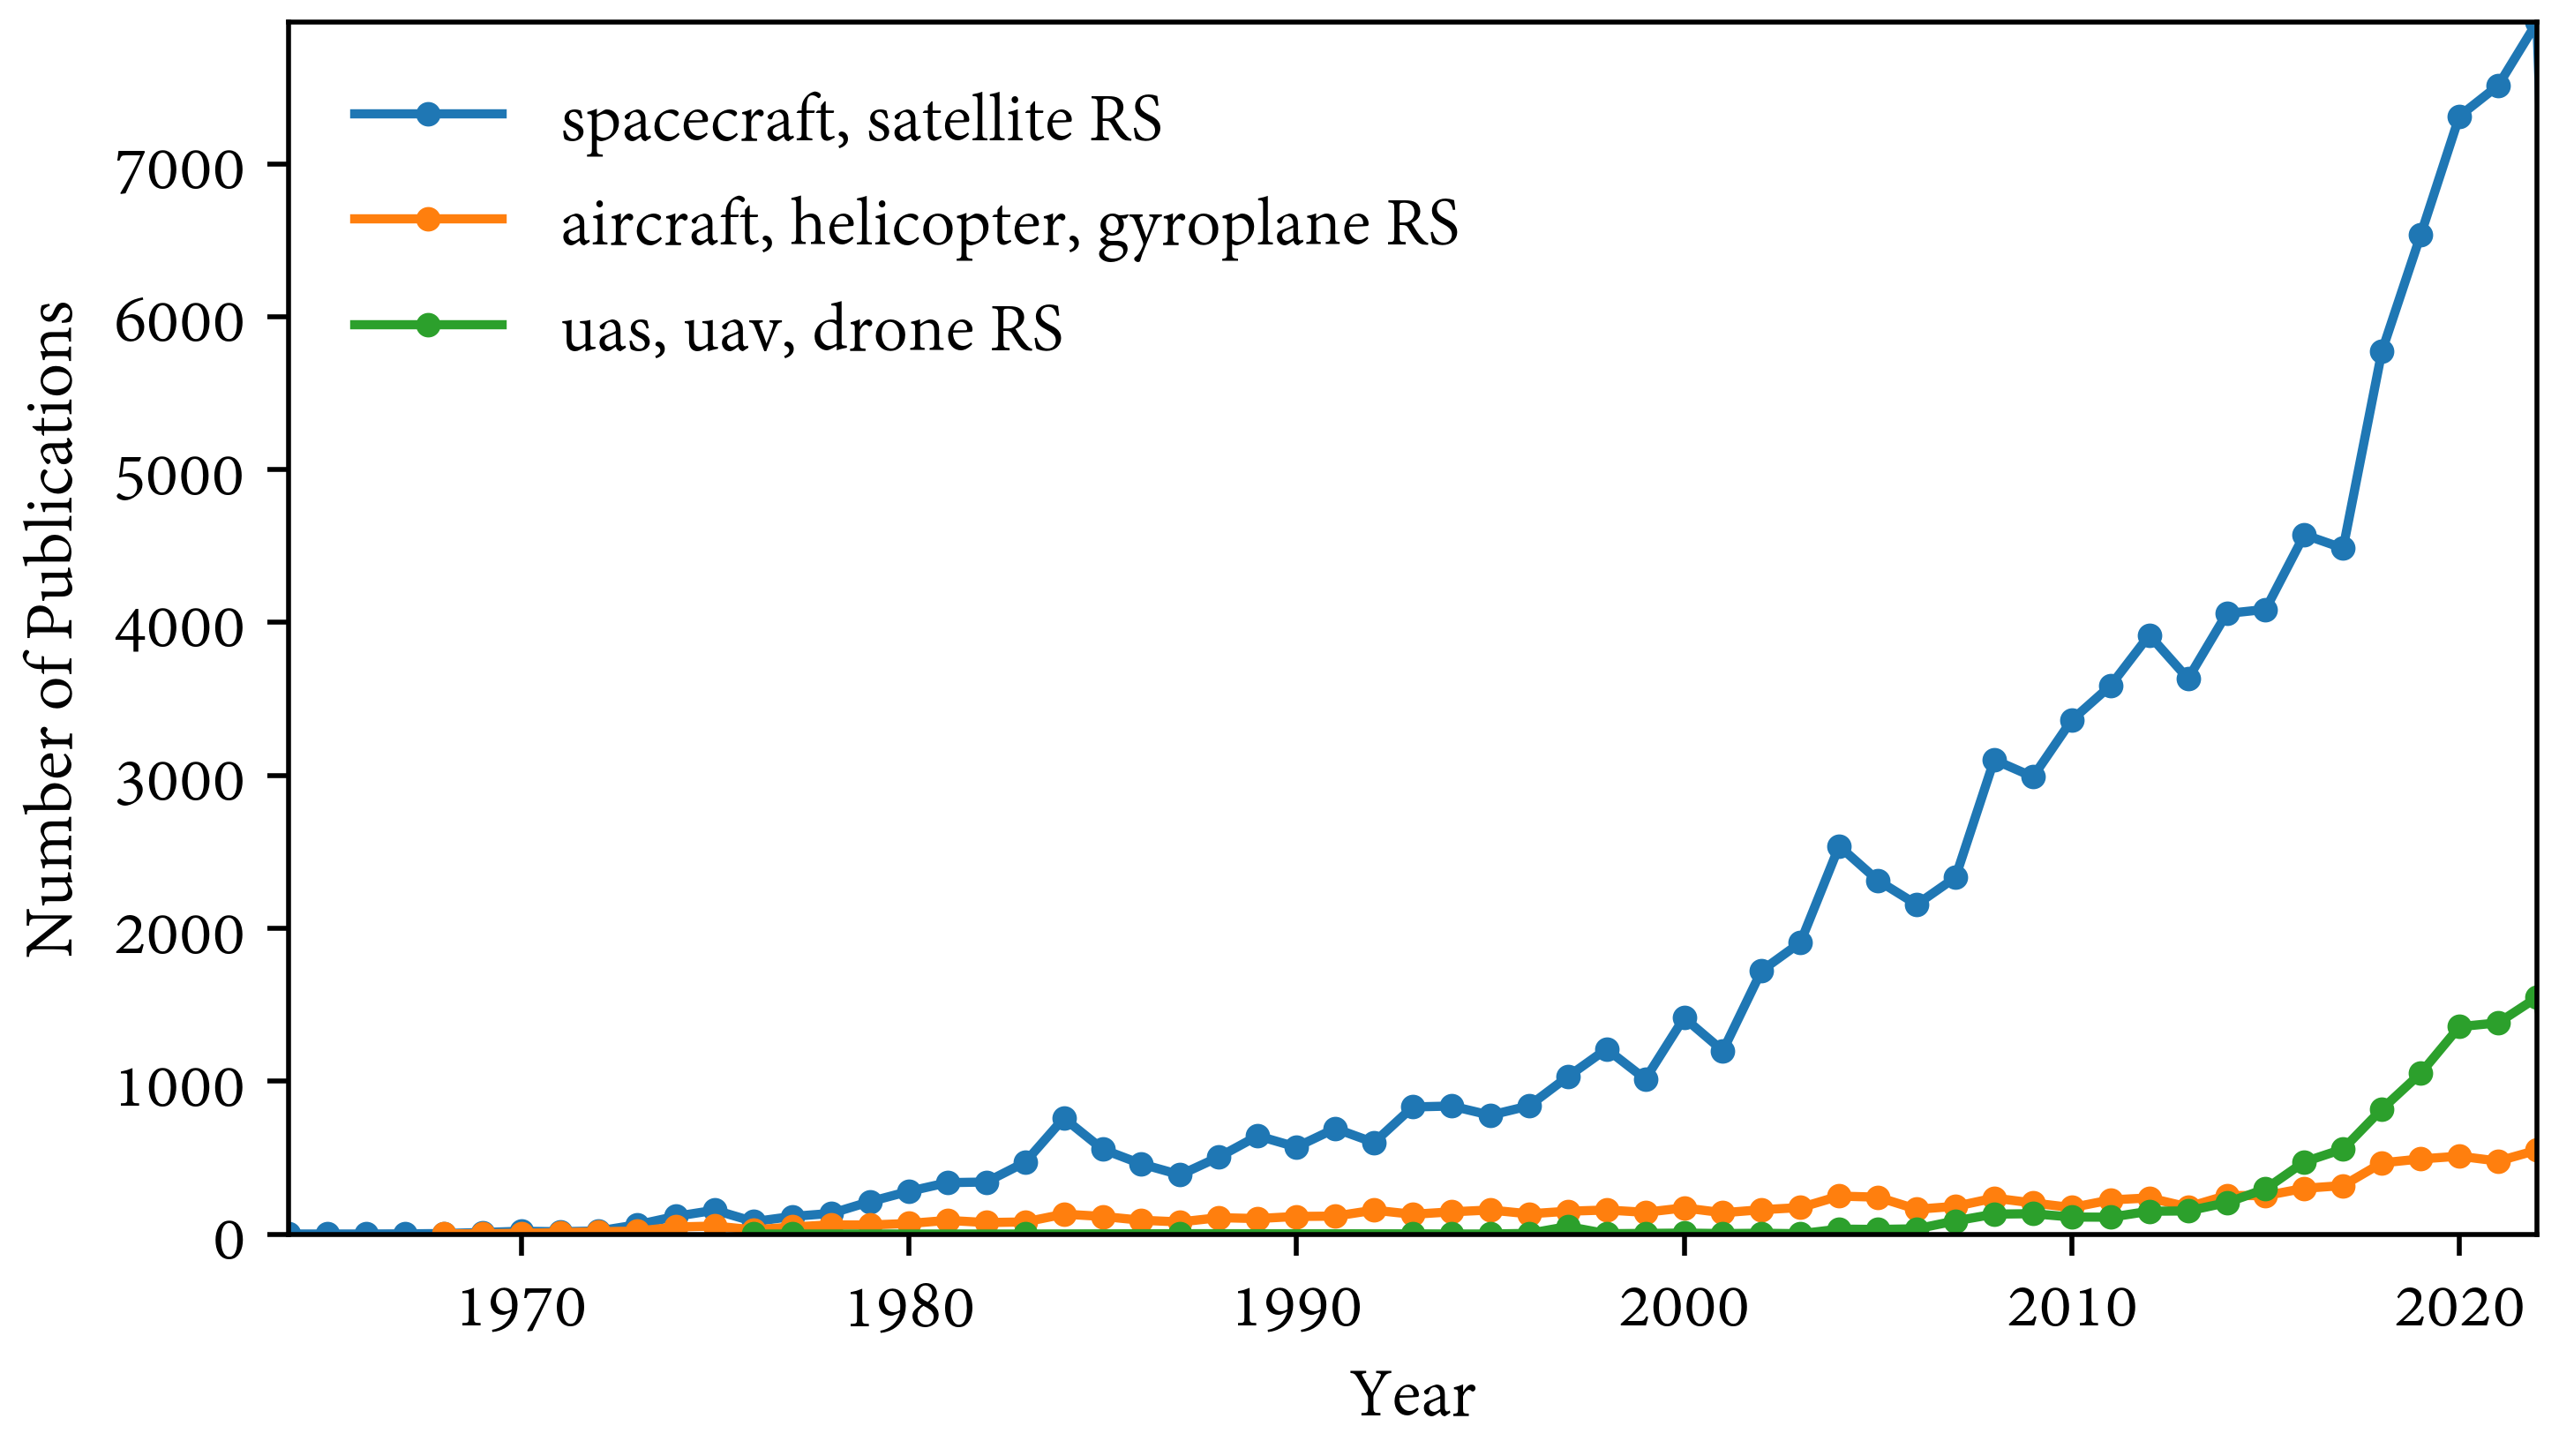
\includegraphics[width=\linewidth]{figs/introduction/platform_timeline.png}
	\caption{Número de artículos relacionados con diferentes plataformas de teledetección. Las búsquedas de Scopus fueran las siguientes: $(p_1 \lor p_2 ... \lor p_n) \land (\textit{remote} \hspace{1mm} \land \hspace{1mm} \textit{sensing})$, donde $p_i$ es una de las plataformas en la leyenda. }
    \label{fig:scopus_search_platforms_spanish}
\end{figure}

\begin{marginfigure}[.7cm]
	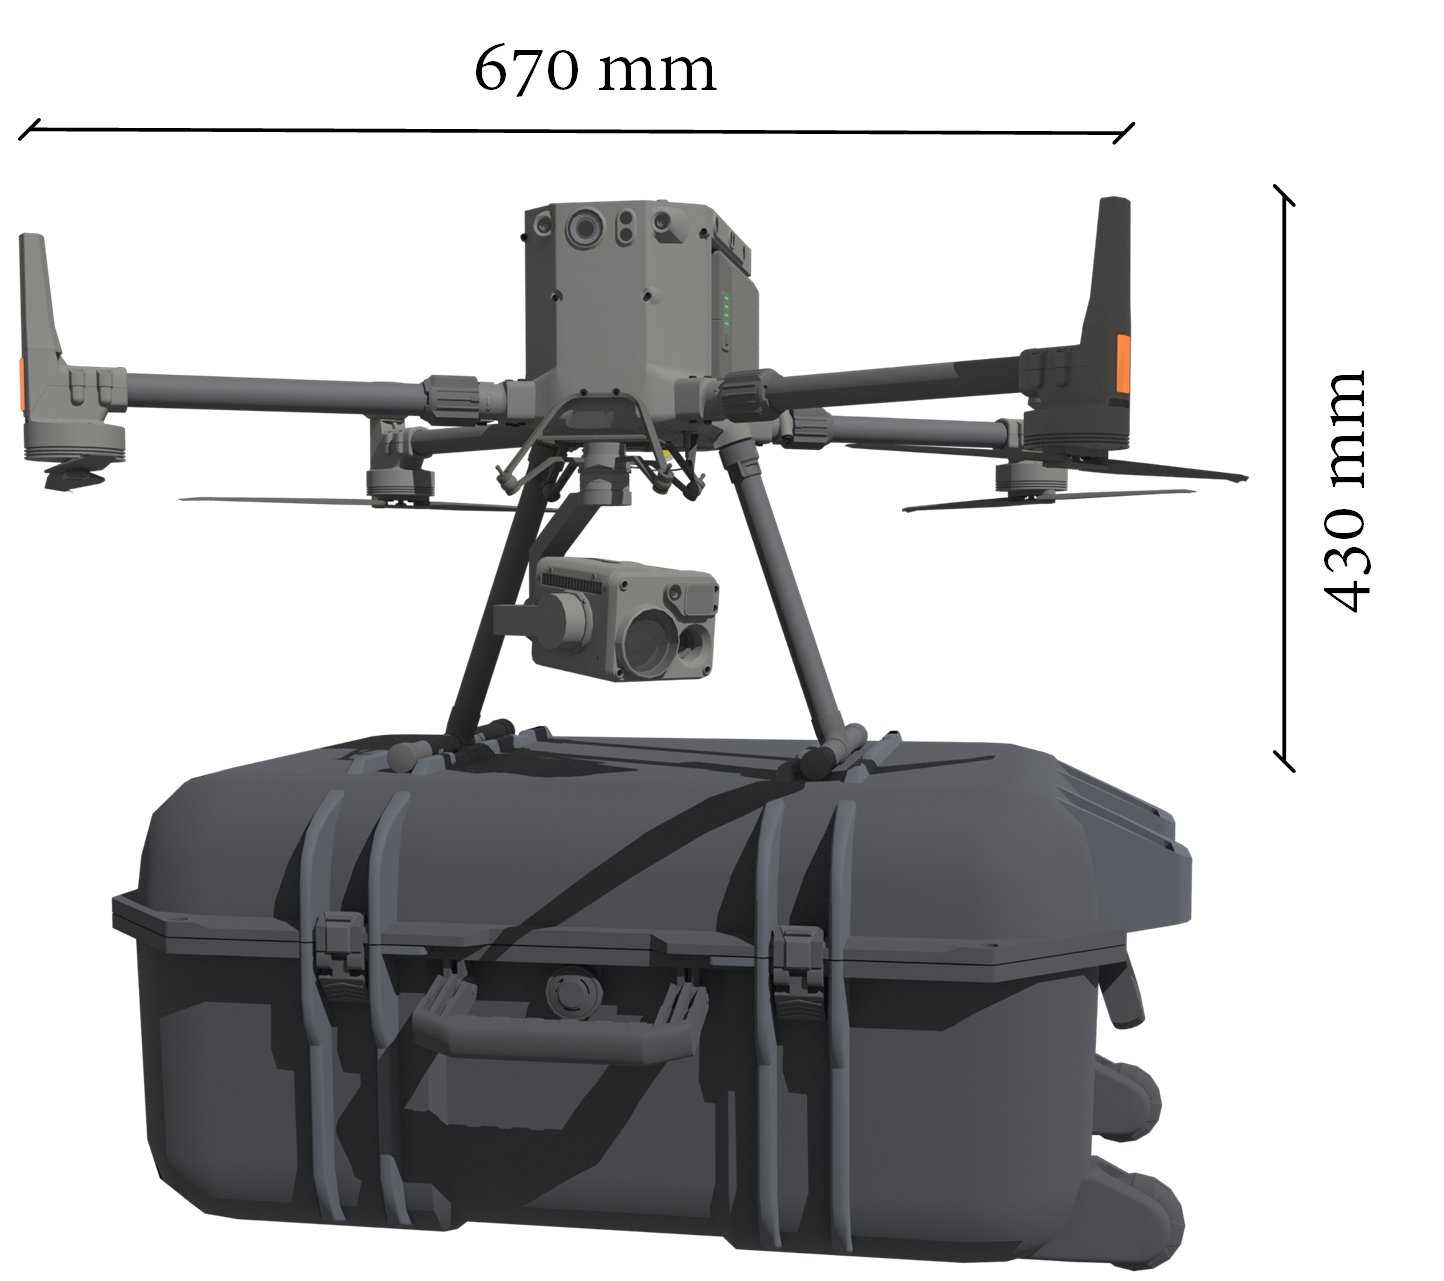
\includegraphics{figs/introduction/dji300.png}
	\caption{Quadcóptero Matrice 300 \acrshort{rtk}, acoplado con un dispositivo dual RGB-termográfico. }
	\label{fig:dji300_spanish}
\end{marginfigure}
Además de las limitaciones técnicas, la resolución de las misiones de satélite se encontraba restringida hasta hace muy poco por algunos gobiernos. Dichas restricciones y limitaciones propiciaron el uso de plataformas alternativas. Además de satélites, \textbf{aeronaves} (ala fija y helicópteros), \textbf{sistemas aéreos no tripulados} (Unmanned Aerial Systems: \acrshort{uas}) (figura \ref{fig:dji300_spanish}) y otras \textbf{plataformas terrestres} (móviles y estáticas con detección próxima) son las más frecuentes en la literatura \cite{lillesand_remote_2015}. La selección de una u otra se deberá sopesar considerando requisitos tales como maniobrabilidad, cobertura terrestre, resolución espacial, precisión espacial, coste y campo de visión (Field of View: \acrshort{fov}). Sin embargo, los vehículos aéreos no tripulados han copado buena parte del interés tanto en investigación como en la industria en la última década. Han pasado de ser simples herramientas militares a principios de la década de los 2000, a sistemas fáciles de desplegar, pequeños y de bajo coste, ampliando así su campo de aplicación a población civil e investigación. Estas plataformas abarcan desde aeronaves del tamaño de una mano a otras de gran tamaño que pueden ser controladas por operadores humanos, o incluso ser parcial o totalmente autónomas. La figura \ref{fig:dji300_spanish} muestra un dron diseñado por DJI que puede transportar hasta 2,7 \si{\kilo\gram}, con unas dimensiones de $501 \times 403 \times 252$ \si{\milli\meter}.

\begin{figure}[!ht]
	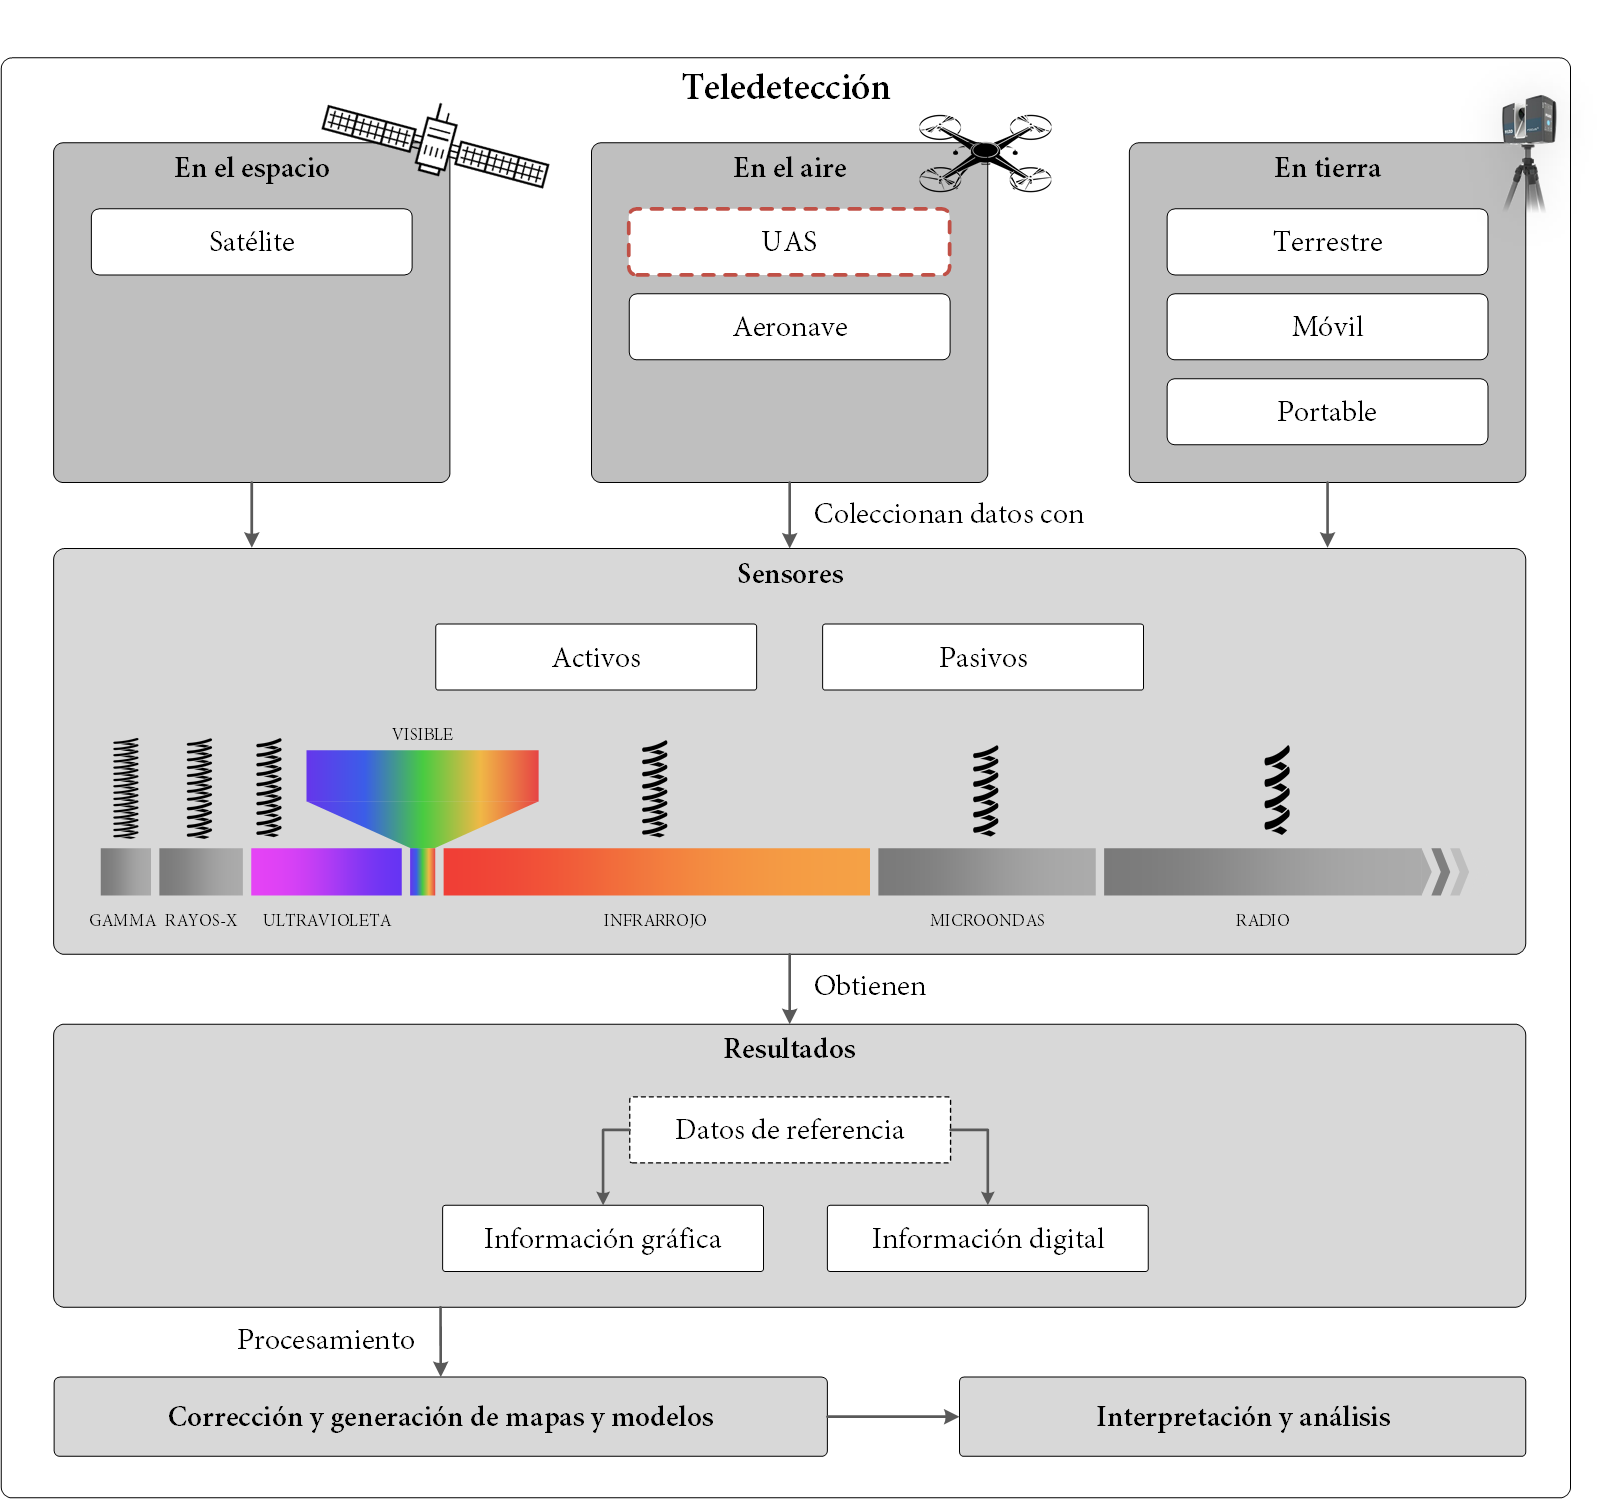
\includegraphics{figs/introduction/introduction_scheme_spanish.png}
	\caption{Procedimiento general de adquisición de datos con plataformas y sensores de teledetección. En primer lugar, los sensores se acoplan en vehículos espaciales, aéreos o terrestres, e incluso pueden ser transportados por humanos. A continuación, se diferencia dos categorías dentro de los productos obtenidos: resultados gráficos y numéricos, aunque la mayoría puede producir ambos tipos de datos. Por último, dichos productos se procesan e interpretan para proporcionar a los usuarios información útil en el control de algún proceso. }
    \label{fig:introduction_scheme_spanish}
\end{figure}

Por tanto, los \acrshort{uas} son vehículos muy económicos para la adquisición de datos de teledetección. Los sensores que más comúnmente se integran son cámaras y sensores \acrshort{lidar} (Light Detection and Ranging), es decir, sensores activos y pasivos, respectivamente. Mientras que los sensores pasivos se basan en una arquitectura transmisor-receptor, los sistemas activos simplemente se limitan a captar la energía emitida por las superficies observadas. Las observaciones de sensores pasivos se materializan en forma de imágenes, mientras que los resultados de un sensor activo son incoporan las tres dimensiones. De esta manera, la \textbf{tecnología activa} es mucho más \textbf{prohibitiva} en términos económicos que cámaras que llevan siendo utilizadas décadas, incluso dando lugar a productos de menor coste dirigidos al público general. En cualquier caso, ambos tipos de tecnología pueden complementarse. Sin embargo, la adquisición de múltiples conjuntos de datos de alta resolución presenta ventajas e inconvenientes. 

\marginnote[.0cm]{La digitalización de objetos, procesos y sistemas se beneficia de las posibles reconstrucciones geométricas que pueden llevarse a cabo mediante la información recabada por sensores. De esta manera, es posible conectar réplicas virtuales y físicas a través de un canal de comunicación. Esto es lo que se conoce hoy en día como gemelo digital.}
En primer lugar, los datos adquiridos por sensores diferentes representan características que forman parte de un \textbf{sistema de conocimiento}, donde cada una de ellas aporta información procedente de un intervalo de longitud de onda distinto. Por tanto, buena parte de los algoritmos dedicados al análisis de datos se pueden ver beneficiados de dichas características complementarias. A pesar de ello, la contribución de todas estas propiedades se podrá ponderar en un proceso de entrenamiento, en función de cómo de importante sean éstas para alcanzar una conclusión. Por tanto, se puede afirmar que es mejor tener un mayor número de características, salvo en aquellos casos en los que son excesivas, dando lugar al llamado problema de la maldición de la dimensionalidad. Además, los datos con una \textbf{resolución elevada} ayudan a generar modelos más \textbf{precisos}, los cuales son mucho más \textbf{fáciles de visualizar y analizar por el ser humano}. La utilización de datos con mayor densidad también deriva en una reconstrucción cuya geometría es mucha más densa, y por ende, omite menos detalles de la escena y facilita la construcción de modelos digitales, simulando procesos y entornos reales. 

En una situación ideal, todas estas capas de información carecen de ruido y se representan en un mismo sistema de coordenadas. Sin embargo, los sistemas de navegación que incorporan los vehículos presentan pequeños errores de posicionamiento que pueden dificultar la fusión de datos. Estos errores se manifiestan en el espacio de la imagen mediante transformaciones relativas de traslación, rotación y escala entre datos de fuentes heterogéneas. Además, las condiciones ambientales, incluyendo composición y partículas, viento, temperatura o radiación solar, pueden variar de un vuelo a otro y por tanto, también los datos adquiridos, a pesar de utilizar planes de vuelo y sensores iguales o similares. Por tanto, estos cambios no sólo afectan a la información adquirida en una misma misión, sino que son especialmente notables en series temporales. No obstante, estas diferencias producidas por errores de posicionamiento y orientación pueden mitigarse mediante el uso de puntos de control. Para ello, se georeferencia un conjunto de puntos con una precisión muy alta, y después, se indica dónde se encuentran representados dichos puntos en la imagen; por tanto, éstos deben ser fácilmente reconocibles. Otros inconvenientes son el ruido procedente de detectores defectuosos, especialmente en el caso de sensores activos, partículas atmosféricas no deseadas o superficies cuyas propiedades reflectivas impiden la observación de una geometría precisa. Todos estos factores evidencian la necesidad de definir un sistema capaz de fusionar con precisión múltiples conjuntos de datos, facilitando así su posterior procesamiento y análisis.

Además de la información adquirida directamente del sensor, pueden ser necesarios otros tipos de datos para tareas de \textbf{visión por computador}. Por ejemplo, \textbf{conocer la etiqueta semántica de un píxel} o un punto 3D sería de gran ayuda para entrenar modelos orientados a la distinción de materiales y objetos. No obstante, es difícil obtener esta información sin incorporar conocimiento previo o sin utilizar modelos ya entrenados con anterioridad. Esto implica que esta tarea se acaba desarrollando en algunos casos por operadores humanos o algoritmos no supervisados que transforman y extraen características relevantes. Sin embargo, ninguno de estos método es perfecto y pueden introducir errores que, en definitiva, derivan en modelos entrenados con datos incorrectos. Por tanto, construir conjuntos de datos de cualquier sensor \textbf{conlleva bastante tiempo}, como resultado de las etapas de adquisición, procesamiento y extracción de características. Todo esto puede evitarse, hasta cierto punto, con conjuntos de datos disponibles en repositorios públicos, los cuales crecen diariamente para dar cabida a algoritmos de Inteligencia Artificial. Éstos cubren un número bastabte amplio de sensores e intervalos de longitudes de onda, pero las propiedades adicionales previamente mencionadas siguen presentando el mismo problema. Además, nada nos garantiza que exista un conjunto de datos para nuestro caso de estudio particular.

Dadas las desventajas de adquirir datos con sensores reales, entre las que destacan el coste de los mismos y el tiempo que consume este proceso, se podría reemplazar total o parcialmente un conjunto de datos con \textbf{información sintética}. Para ello, se modela un \textbf{sensor virtual} que debe simular el comportamiento del sensor real. De esta manera, se puede añadir mucho más conocimiento en cada primitiva y se puede resolver la tarea de generación de conjuntos de datos en mucho menos tiempo. Esta tarea requiere escenarios sintéticos cuyos modelos no presentan incertidumbre alguna, y por tanto, se pueden vincular estos con propiedades, como la etiqueta semántica, que en última instancia se transfieren a los datos adquiridos por el sensor virtual. Se evita así el coste de adquirir sensores tan prohibitivos como la tecnología \acrshort{lidar}. En la literatura, los sensores más comúnmente simulados son Radar y \acrshort{lidar}, aunque los últimos avances en Deep Learning (\acrshort{dl}) también posibilitan la generación de imágenes sintéticas.

Los conjuntos de datos obtenidos con anterioridad suelen \textbf{transformarse} en otros tipos de \textbf{representaciones derivadas}, pero no obtenidas de manera directa de un sensor. Por ejemplo, la identificación de anomalías térmicas podría no ser lo suficientemente trivial en el ámbito de la imagen, especialmente para situar dichas anomalías en un escenario. Una visión mucho más completa e intuitiva se deriva del ámbito de la imagen en forma de mapas 2D y nubes de puntos 3D. Estos resultados pueden calcularse estimando la posición y orientación de los diferentes puntos de adquisición, así como mediante la búsqueda de características comunes en varias imágenes. Durante esta transformación, las propiedades radiométricas y geométricas estimadas pueden sufrir una pérdida de precisión importante a consecuencia de la interpolación de datos, por lo que puede medirse la precisión de este proceso comparando con otros tipos de datos más fiables. Por ejemplo, las nubes de puntos \acrshort{lidar} obtienen una geometría mucho más precisa que podría utilizarse para evaluar la calidad de las nubes de puntos reconstruidas mediante imágenes. Del mismo modo, las propias imágenes pueden utilizarse para medir la calidad de la información radiométrica derivada.   

Por otro lado, \textbf{los grandes volúmenes de datos dificultan el procesamiento, el almacenamiento y la visualización de datos}. No es sencillo procesar miles de imágenes, o grandes nubes de puntos, en ordenadores destinados a un público general, los cuales suelen disponer de un almacenamiento muy restringido y unas capacidades de cómputo no orientadas a ofrecer un alto rendimiento. A pesar de esto, es más común encontrar hoy en día ordenadores personales y profesionales con una elevada capacidad de almacenamiento, un acceso más eficiente a datos y una mayor capacidad de cómputo y paralelismo. Este último factor dependerá de la Unidad Central de Procesamiento (Central Processing Unit: \acrshort{cpu}), cuya tendencia es aumentar el número de núcleos, y de la Unidad de Procesamiento Gráfico (Graphics Processing Unit: \acrshort{gpu}), compuesta por millones de pequeñas unidades que permiten resolver tareas muy simples con un paralelismo masivo, así como intercambiar datos entre diversos hilos de manera eficiente. La sección \ref{sec:data_types} profundiza en los formatos de datos más comunes en teledetección; por ahora, basta con hacernos una idea de que estos datos son simplemente millones de números (Digital Number, \acrshort{dn}). A pesar de que hoy en día el almacenamiento presenta un coste mucho más reducido, algunos inconvenientes aún persisten, como la recuperación eficiente y parcial de información almacenada, especialmente en aplicaciones interactivas \cite{bejar-martos_strategies_2022, ogayar-anguita_nested_2023}. 

Otro inconveniente de las aplicaciones en tiempo real es la \textbf{visualización de grandes volúmenes de datos}. Los métodos tradicionales de rendering contienen un conjunto de etapas predefinidas, en las que la geometría y la topología del modelo se transforman iterativamente para producir una imagen compuesta por píxeles. Los colores de éstos se calculan considerando la influencia de una o varias fuentes de luz sobre las texturas de una superficie, discretizando así la formulación que describe la interacción de la luz con la escena. A diferencia de los modelos sintéticos diseñados por el ser humano, los datos obtenidos por sensores reales se sombrean en función de la radiancia observada en un conjunto de longitudes de onda a las que es sensible el dispositivo. Por tanto, son necesarias metodologías de visualización de datos mucho más flexibles, evitando así algunas etapas innecesarias, como el sombreado de primitivas. De acuerdo con la arquitectura de una \acrshort{gpu}, los datos pueden ordenarse y organizarse en estructuras de datos que permiten balancear dos factores: carga de trabajo y precisión geométrica. Ésta última permite alterar la percepción del usuario si se realiza en su justa medida. Además, estas restricciones son aún más mayores en aplicaciones de Realidad Virtual (\acrshort{vr}) que sombrean la escena al menos dos veces, una por cada ojo, e incluso puede incrementarse aún más en función de las técnicas de iluminación empleadas.
\begin{marginfigure}[-7.5cm]
	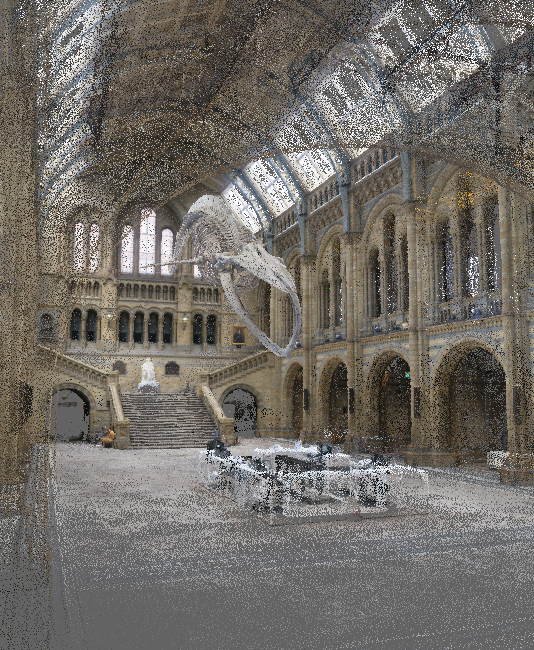
\includegraphics{figs/introduction/hintze.png}
	\caption{Nube de puntos con 2.4M de puntos reconstruidos utilizando 900 imágenes adquiridas en la Sala Hintze (Modelo de \textit{Thomas Flynn} en \textit{Sketchfab}).  }
	\label{fig:hintze_hall_spanish}
\end{marginfigure}

\marginnote[1cm]{Esta tesis tiene como principal campo de aplicación la Agricultura de Precisión y por tanto, el análisis de datos se ha acotado a 1) segmentar cultivos, y 2) clasificar variedades de éstos de manera no destructiva.}
Los métodos anteriores no son más que un procedimiento para extraer información textual o visual a partir de datos de sensores. En consecuencia, el \textbf{último paso} es la \textbf{clasificación, segmentación e identificación de características} a partir de los datos de entrada. Las principales aportaciones de las técnicas de teledetección en la Agricultura de Precisión son la estimación del rendimiento de una plantación, la clasificación del tipo de cultivo, la medición del agua disponible, el índice de área foliar (Leaf Area Index, \acrshort{lai}) o el control de enfermedades e insectos, así como la monitorización de humedad, cambios, crecimiento, estrés y falta de agua, además de otros factores de riesgo como la nieve o el fuego \cite{huang_agricultural_2018}. Con estas tareas de vigilancia se pretende maximizar la rentabilidad y minimizar los residuos y la contaminación. 

\section{Contexto histórico y tecnología}

El término \textbf{teledetección} se originó en la década de 1960, acuñado por Eveleyn Pruitt para referirse a instrumentos satelitales y aéreos que posibilitaban medir la radiancia reflejada y emitida. Por otro lado, las técnicas topográficas fueron inicialmente diseñadas en 1849, y llevadas a la práctica en 1858 por F. Tournachon en un globo aerostático que sobrevoló Francia. A partir de aquí, el tamaño de las cámaras se ha ido reduciendo para hacerlas más cómodas de manejar. Otros medios aéreos empleados para una teledetección temprana, ya fueran producto de la investigación o de acontecimientos históricos tales como guerras, fueron cometas (1906; Figura \ref{fig:san_francisco_kite_spanish}), aves (1909) y aeronaves (1908). 

\begin{figure}[!ht]
	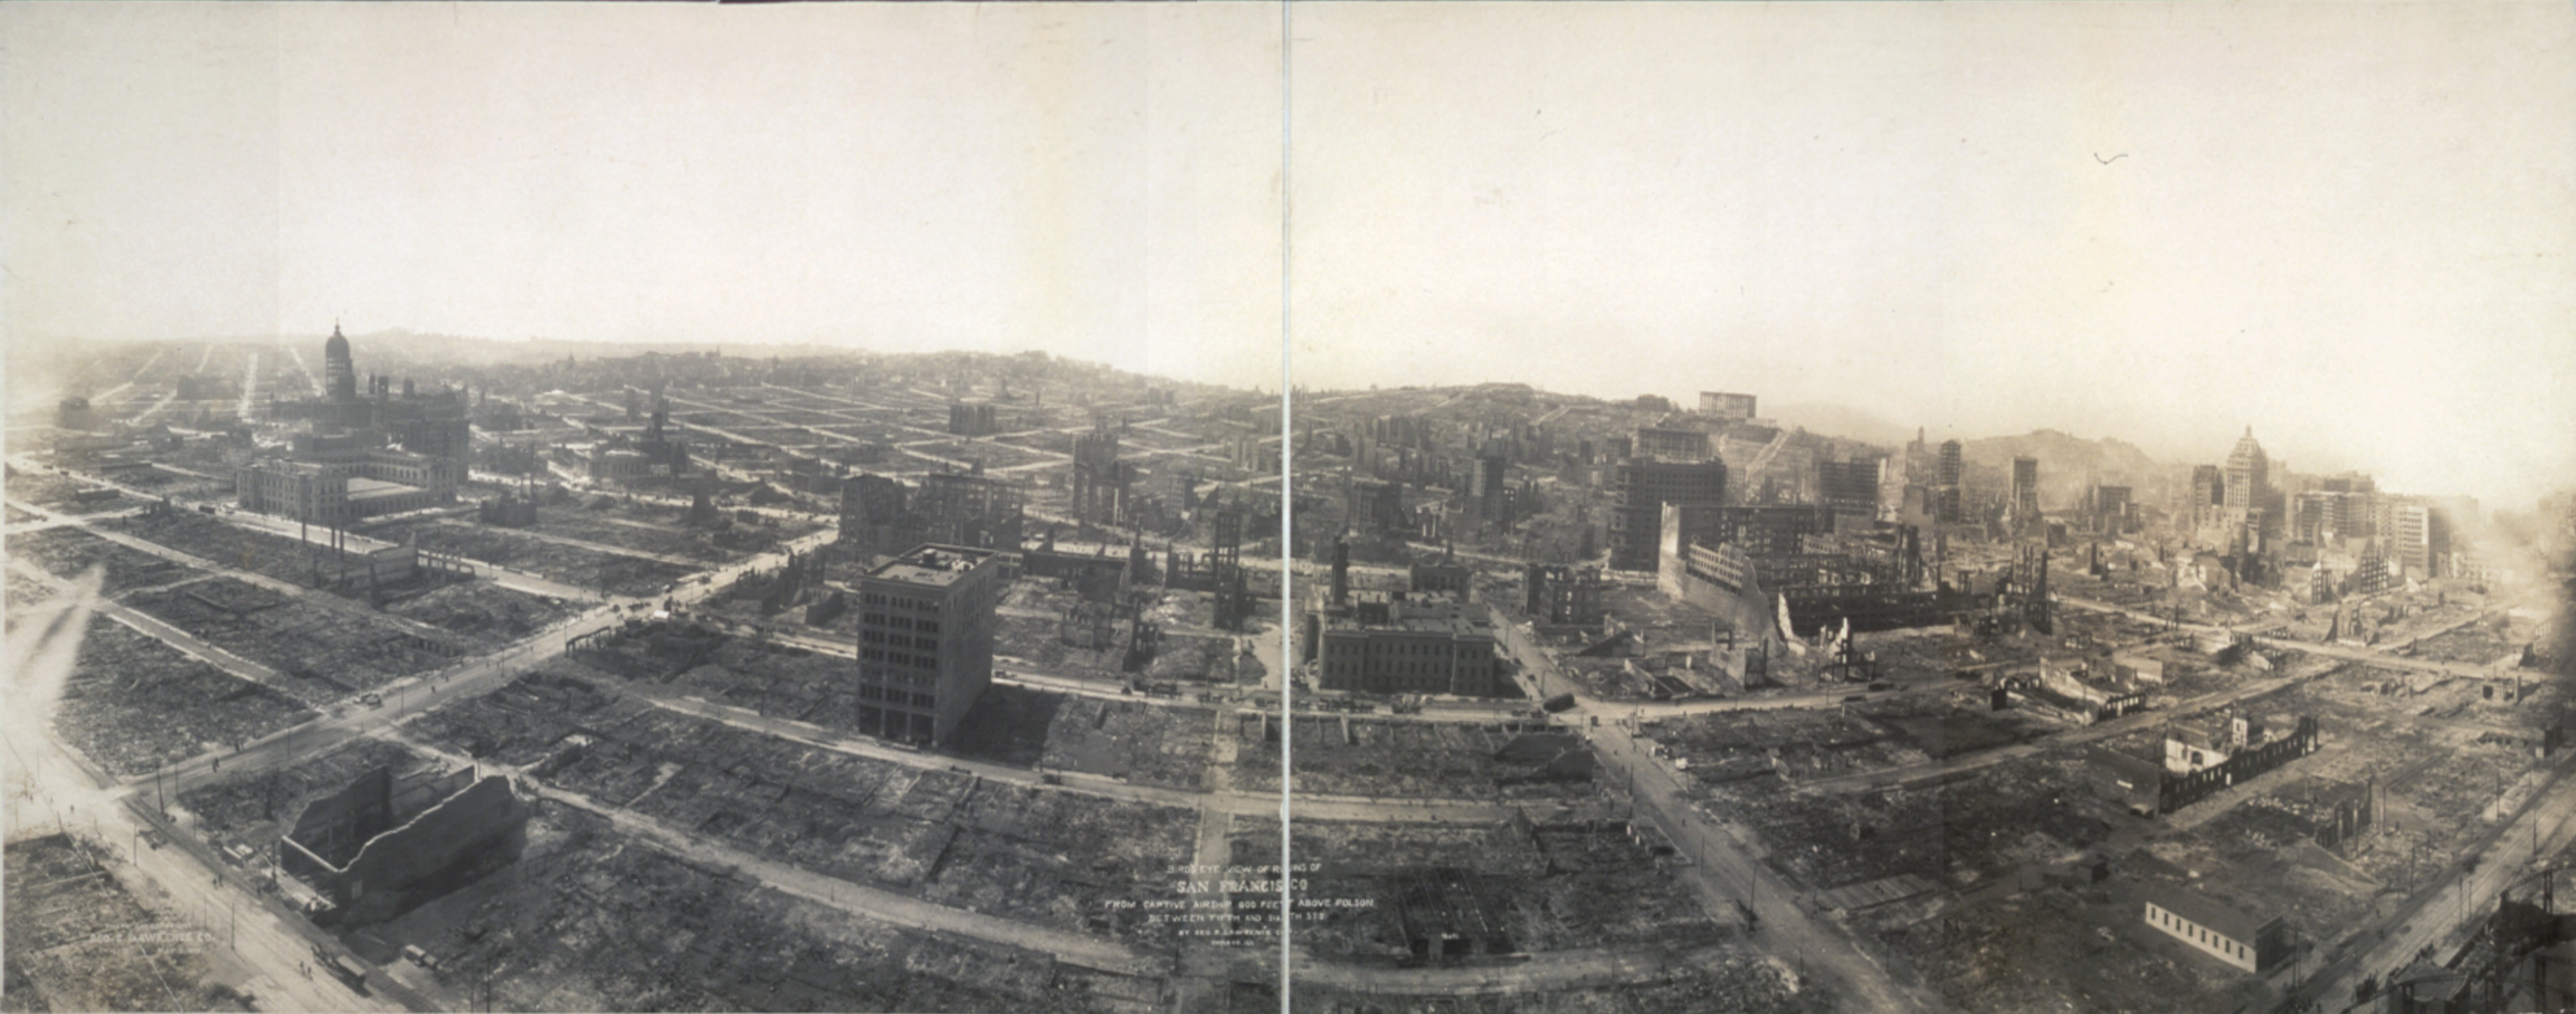
\includegraphics[width=0.95\linewidth]{figs/introduction/san_francisco_kitecamera.jpg}
	\caption{Fotografía de San Francisco después del terremoto de 1906, capturada desde una cámara soportada por siete cometas. }
    \label{fig:san_francisco_kite_spanish}
\end{figure}

La teledetección mediante satélite, tal y como se conoce hoy en día, es posible gracias a la idea inicial de Konstantin Tsiolkovsky de utilizar cohetes para explorar el espacio, publicada bajo el título \textit{Exploring Space using jet propulsion devices}. Esta idea se vio finalmente realizada con el primer lanzamiento con éxito de un satélite, el Sputnik (1957), e igualmente contribuyó al desarrollo de satélites destinados a la vigilancia atmosférica. El satélite de observación por televisión e infrarrojos (Television and Infrared Observation Satellite: \acrshort{tiros}) entró en funcionamiento en 1960, integrando un pequeño sistema infrarrojo y una cámara sensible al espectro visible con un ángulo de visión muy reducido. En 1978, \acrshort{tiros}-N (n haciendo referencia a "new") supuso un antes y un después tanto en la plataforma como en los sensores. Esta misión integraba un radiómetro con una resolución de 1 \si{\kilo\meter} que podía capturar información en el espectro visible, infrarrojo cercano, infrarrojo medio e infrarrojo lejano. En la actualidad, una versión más avanzada de este satélite opera con el nombre de \acrshort{avhrr} (Advanced Very High-Resolution Radiometer), con una resolución similar y capacidad para capturar seis bandas espectrales diferentes, en lugar de sólo cuatro \cite{national_oceanic_and_atmospheric_administration_avhrr3_nodate}.   

\marginnote[.1cm]{Un amplio repositorio de misiones de satélite se encuentra disponible en el Earth Observation Portal perteneciente a la Agencia Espacial Europea \cite{earth_observation_portal_earth_nodate}.} 
Entre los proyectos de satélite actualmente operativos, Landsat es el que proporciona la mayor cantidad de datos de teledetección que se han adquirido de manera continuada. Tuvo su origen formando parte del programa NIMBUS de la NASA, y en la actualidad hay dos satélites activos, Landsat 8 y Landsat 9, mientras que los otros siete han sido desmantelados o está previsto en los próximos años (por ejemplo, esto último ocurre con Landsat 7). La misión Landsat 9 consta de dos sensores: Operational Land Imager (\acrshort{oli2}) y un sensor infrarrojo térmico (\acrshort{tirs2}). Cada día obtiene un total de 740 escenas en 11 intervalos espectrales diferentes, incluyendo rojo, azul, verde, infrarrojo cercano, infrarrojo de onda corta, lejano, pancromático, costero y de cirros, con una resolución que oscila entre 15 \si{\meter} y 100 \si{\meter}. Otras misiones de satélite destacadas son el Satélite de Recursos Terrestres China-Brasil (China–Brazil Earth Resources Satellite: \acrshort{cbers}) y el programa Copernicus, financiado por la Comisión Europea. El satélite CBERS-04A está equipado con tres sensores que capturan cinco intervalos diferentes con una resolución espacial entre 2 \si{\meter} y 55 \si{\meter} \cite{instituto_nacional_de_pesquisas_espaciais_inpecbers_2019}. Por su parte, la misión Sentinel-2 es capaz de obtener datos en 13 bandas distribuidas en el espectro visible, infrarrojo cercano e infrarrojo de onda corta (ver Figura \ref{fig:sentinel2_spanish}), con una resolución espacial que oscila entre 10 \si{\meter} y 60 \si{\meter} \cite{european_environment_agency_eu_2017}. El periodo de tiempo para revisitar el mismo punto de la Tierra es de diez días, en comparación con los 16 días que necesita Landsat 9 o los 31 días de CBERS-04A.

\begin{figure}[!ht]
	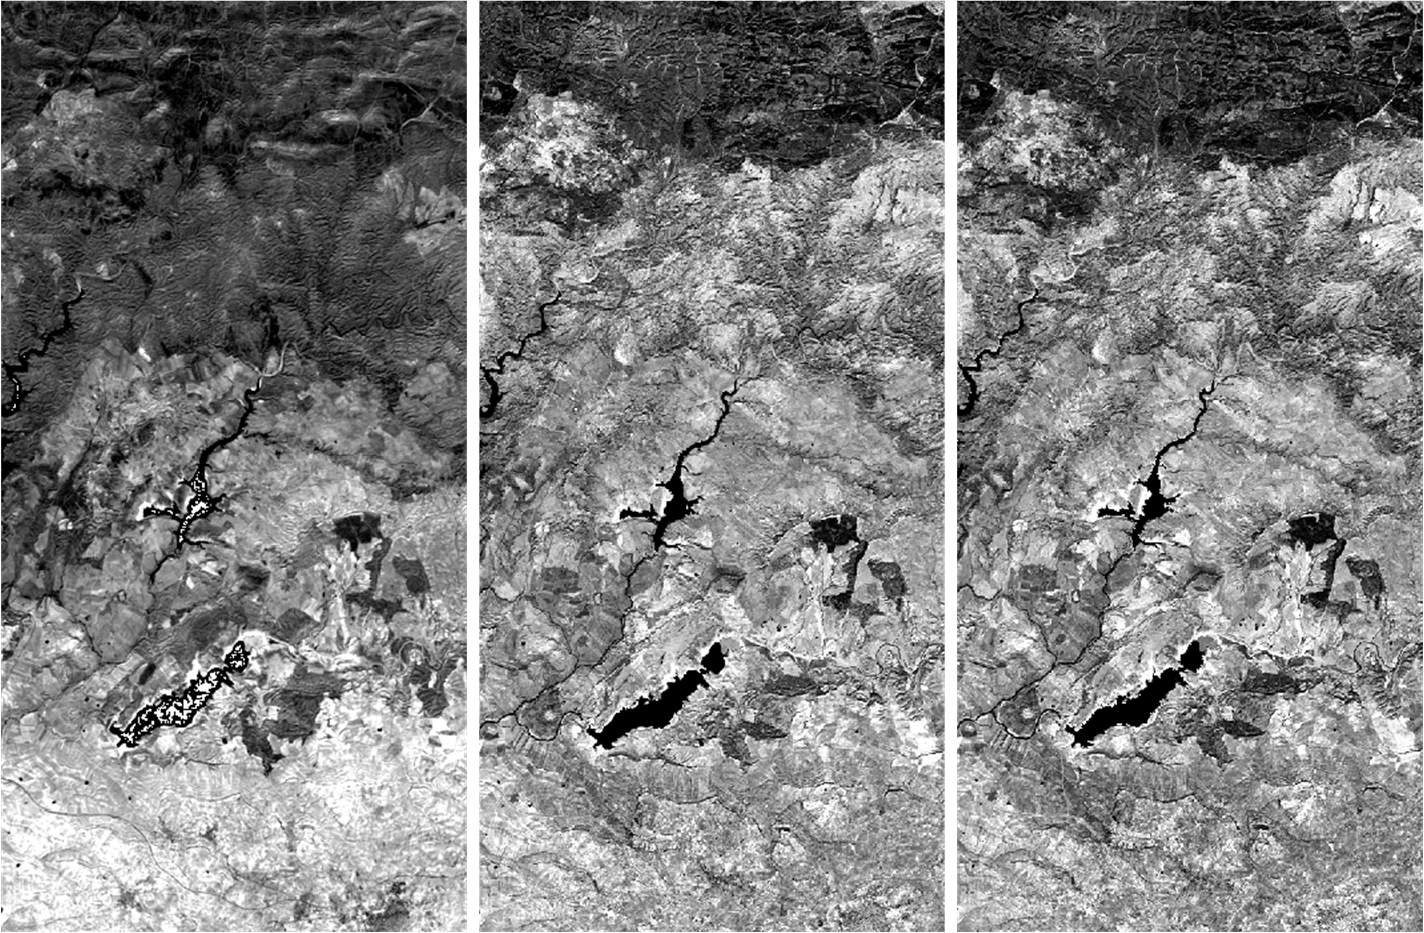
\includegraphics{figs/introduction/sentinel2_bands.png}
	\caption{Tres bandas en el infrarrojo cercano capturadas por la misión Sentinel-2 (banda 9, 935-955 \si{\micro\meter}, banda 11, 1567-1658 \si{\micro\meter}, y banda 12, 2114-2889 \si{\micro\meter}). }
    \label{fig:sentinel2_spanish}
\end{figure}

As observed, the main limitations of satellite datasets are their temporal and spatial resolution. However, these drawbacks are being mitigated nowadays, especially by commercial missions. For instance, the commercial satellite Pléiades Neo (VHR-2020) from Airbus Defense \& Space \cite{airbus_pleiades_2021} is able to daily acquire seven bands with a \acrshort{gsd} of up to 30 \si{\centi\meter} for panchromatic images. Even for governmental missions, the repeat cycle is typically reduced as several twin missions could be active at the same moment with similar instruments and orbits. Accordingly, the offset in Landsat-8 and Landsat-9 trajectories allows acquiring data from the same point every 8 days \cite{masek_landsat_2020}. On the other hand, spatial resolution is steadily improving as most governmental restrictions have been lifted. Yet, spaceborne platforms are the most expensive Remote sensing technology by a huge lead. 

Por tanto, las principales limitaciones de la observación mediante satélite son su resolución temporal y espacial. No obstante, dichos inconvenientes se están mitigando en la actualidad, especialmente en misiones comerciales. Por ejemplo, el satélite comercial Pléiades Neo (VHR-2020) de Airbus Defense \& Space \cite{airbus_pleiades_2021} es capaz de adquirir diariamente siete bandas con una resolución de 30 \si{\centi\meter} por píxel. Incluso en misiones financiadas por entidades públicas, el periodo de repetición se reduce a menudo debido a la existencia de diversas misiones complementarias que operan con órbitas y sensores similares. De esta manera, las misiones Landsat 8 y Landsat 9 obtienen datos de un mismo punto cada 8 días \cite{masek_landsat_2020}. Aun así, acceder a datos de satélite con una resolución elevada es mucho más prohibitivo en comparación con otras técnicas.

Además de la observación mediante satélite, el uso de \acrshort{uas} ha aumentado considerablemente en la última década, atrayendo así el interés tanto de la industria como de la investigación. Los componentes más frecuentes de un \acrshort{uas} son sensores ópticos así como sistemas de navegación y comunicación. Estos últimos permiten al operador desplazar la plataforma dentro de un rango de comunicación, y transferir datos en un canal bidireccional. Independientemente de la ruta de navegación, ya sea manual o establecida mediante algunos puntos de control, se emplean Sistemas de Posicionamiento Global (Global Positioning System: \acrshort{gps}) y Unidades de Medición Inercial (Inertial Measurement Unit: \acrshort{imu}) para calcular y registrar la posición, orientación y movimiento de la nave. Estos componentes son especialmente relevantes para realizar misiones con un alto grado de precisión, la cual se indica mediante el error vertical y horizontal en metros (\si{\meter}). En este sentido, las últimas series de drones de DJI incluyen en sus especificaciones errores verticales y horizontales por debajo del metro, utilizando posicionamiento cinemático en tiempo real en lugar de \acrshort{gps}. Como cabría de esperar, aquellos drones que integran sistemas de navegación más ligeros y más precisos también son más prohibitivos.    

En términos de normativa de seguridad, el término \acrshort{uas} no sólo se refiere al propio vehículo, sino también a los sensores acoplados. Los sensores que suelen integrarse en vehículos aéreos varían en función de la altitud de vuelo y la velocidad de la plataforma, así como de los requisitos del caso de estudio. Los vehículos de ala fija y rotatoria están mucho más limitados en altura y velocidad respecto de otras plataformas tales como helicópteros y autogiros. Aparte de las propias limitaciones de la plataforma, la altitud de vuelo puede estar limitada por normativa para evitar entrar en el dominio aéreo de otros vehículos. Por ello, los sensores y las misiones que requieren menor velocidad, menor altitud de vuelo y, por tanto, mayor precisión, son especialmente convenientes para drones. Un ejemplo muy extendido de esto mismo en teledetección es la monitorización de torres y líneas de transmisión, éstas últimas con una estructura muy fina. Por tanto, este caso de estudio requiere un proceso de toma de datos mucho más lento. En comparación, otras tecnologías, como \acrshort{insar} (Interferometric Synthetic Aperture Radar), se han aplicado principalmente a misiones espaciales para rastrear cambios en la superficie terrestre.
\marginnote[-3.0cm]{La operabilidad de las aeronaves no tripuladas en la Unión Europea está regulada por el reglamento 2019/947. Entre otras restricciones, la altitud máxima de vuelo se limita en 120 \si{\meter} sobre la superficie terrestre, salvo que sobrevuele un obstáculo.} 

\section{Propósitos y objetivos}

Dados los problemas planteados, el objetivo de esta tesis es contribuir en algunas de las etapas presentadas en la Figura \ref{fig:introduction_scheme_spanish}, tales como la fusión y el análisis de información. De entre todos los problemas presentados, destaca la adquisición de conjuntos de datos heterogéneos, la corrección geométrica y radiométrica de datos, así como la fusión de los mismos, la generación de productos de mayor dimensionalidad (por ejemplo, pasando del 2D al 3D) o el análisis de los conjuntos de datos. Acorde a estos problemas, los objetivos específicos de esta tesis son los siguientes:
\begin{itemize}
    \item Corrección y procesamientos de datos adquiridos desde dron. Este objetivo implica corregir tanto los errores geométricos como radiométricos en el espacio de la imagen. Las distorsiones geométricas deben resolverse en la mayoría de escenarios, dado que posibilita la fusión de datos, mientras que las correcciones radiométricas podrán llevarse a cabo o no en función del uso posterior del conjunto de datos. 
    \item El registro de imágenes obtenidas mediante sensores diferentes, eliminando así las diferencias provocadas por la 1) distancia temporal que pudiera existir en el instante de captura, 2) posibles defectos ópticos del sensor, 3) la arquitectura del propio sistema óptico y 4) el intervalo de longitudes de onda adquirido. La fusión de imágenes debe resolverse sobre imágenes que presentan valores de intensidad muy diferentes, al corresponderse a longitudes de onda diferentes. Se obtiene pues, como resultado de esta fusión, una matriz de transformación que permite la proyección de unos datos en otros.
    \item Generación de nubes de puntos 3D muy densas en un reducido tiempo de respuesta, con varias capas procedentes de diversos conjuntos de datos. La metodología debe eliminar algunos de los errores más comunes en la fotogrametría, como la presencia de errores geométricos, el elevado tiempo de respuesta, etc. Dado el gran volumen de puntos que debe abordarse, y la presencia de múltiples fuentes de datos, la generación de nubes debe plantearse mediante un enfoque de computación paralela.
    \item Los conjuntos de datos previamente adquiridos desde dron carecen de información adicional que pudiera ser relevantes para aplicaciones de Inteligencia Artificial, como la etiqueta semántica de cada punto o píxel. Al elevado tiempo que conllevaría añadir este tipo de datos de forma manual, se debe añadir el tiempo derivado de la adquisición, la corrección y el procesamiento de datos. Además, existen sensores tales como \acrshort{lidar} cuyo coste es mucho mayor que el de otros sensores, por ejemplo, cámaras térmicas o multiespectrales. Por tanto, es posible sustituir de manera parcial, o completa, conjuntos de datos obtenidos por sensores reales por información generada mediante un sensor virtual. Dicha herramienta debe simular el comportamiento del sensor real desde un punto de vista geométrico y radiométrico. Además, se trata de una tarea con un elevado coste computacional, y por tanto, debe implementarse de manera eficiente y haciendo uso de paralelismo. Por otro lado, tampoco es trivial estimar la intensidad capturada, razón por la cual deben caracterizarse las superficies modeladas en el escenario sintético.
    \item Por último, los productos previamente adquiridos, procesados o generados deben de tener un fin último, plasmado en una aplicación. Entre ellas se encuentra la detección de anomalías térmica en restos arqueológicos, la clasificación de variedades de vegetación o la planificación de sesiones de adquisición de datos \acrshort{lidar}. Puede llevarse a cabo mediante técnicas tradicionales, por ejemplo, basadas únicamente en la geometría del entorno, o utilizando modelos de Inteligencia Artificial.
\end{itemize}

\section{Organización del documento}

\newcommand{\partSpacing}{1mm}

Esta tesis se compone de seis partes diferentes:

\small \textbf{\textls[30]{PARTE I}} \normalsize\hspace{\partSpacing} Esta parte abarca el capítulo actual, donde se introduce la terminología básica de teledetección, al mismo tiempo que se plantean algunos de los principales retos de dicha área. Después, el Capítulo \ref{sec:fundamentals_rs} presenta una descripción mucho más amplia de los principales sensores, productos obtenidos y tareas de procesamiento. Por último, el Capítulo \ref{sec:context_rs} contiene la revisión del estado del arte de la fusión de datos adquiridos desde dron, y la simulación de éstos.

\small \textbf{\textls[30]{PARTE II}} \normalsize\hspace{\partSpacing} En esta parte se detallan los conceptos básicos de este trabajo, incluyendo qué tipo de sensores y datos se utilizan. Después, se describe el proceso de corrección y fusión de imágenes sobre el que se sustenta buena parte de este trabajo. Por tanto, esta sección engloba tanto materiales como métodos que serán utilizados en capítulos posteriores.

\small \textbf{\textls[30]{PARTE III}} \normalsize\hspace{\partSpacing} Esta parte presenta la generación eficiente de nubes de puntos 3D compuestas por múltiples capas: información en el espectro visible, infrarrojo lejano, multiespectral e hiperespectral. La información visible servirá para generar una nube de puntos 3D de referencia, sobre la cual se proyectará el resto de información. Esto implica el registro de diversas fuentes de información y su posterior proyección en la nube mencionada. Además, dado el tiempo de respuesta necesario, se puede llevar a cabo este proceso en la tarjeta gráfica con el fin de acelerar el proceso. 

\small \textbf{\textls[30]{PARTE IV}} \normalsize\hspace{\partSpacing} El procesamiento de algunos conjuntos de datos, como LiDAR o nubes de puntos estimadas con fotogrametría, no es trivial ni eficiente en términos de recursos humanos y computaciones. Por ejemplo, podríamos necesitar etiquetas semánticas sobre los conjuntos de datos previos. Por otro lado, sensores tales como LiDAR son bastante más prohibitivos económicamente que las cámaras empleadas en Parte III. En esta sección, se propone una herramienta de simulación \acrshort{lidar} sobre escenarios sintéticos, enfocada en 1) la estimación de las propiedades geométricas de una nube de puntos \acrshort{lidar} (Capítulo \ref{sec:lidar_simulation}) y 2) el cálculo de la radiancia observada (Capítulo \ref{sec:lidar_intensity}). 

\small \textbf{\textls[30]{PARTE V}} \normalsize\hspace{\partSpacing} En esta parte se incluyen algunas aplicaciones derivadas del procesamiento de nubes de puntos térmicas e imágenes hiperespectrales, así como de la simulación de escaneos LiDAR. La primera aplicación será la detección de anomalías térmicas en yacimientos arqueológicos. Por otro lado, la información hiperespectral se aplicará a la identificación automática de variedades de viñedos, utilizando modelos de Inteligencia Artificial. Finalmente, la simulación \acrshort{lidar} se aplica en la optimización de escaneos terrestres, con el fin de indicar qué posiciones son las óptimas de acuerdo a la configuración del sensor. Este proceso de optimización se describe en el Capítulo \ref{sec:lidar_optimization} y se orienta principalmente a edificios, aunque no presenta restricciones que impidan su aplicación en otros ámbitos.

\small \textbf{\textls[30]{PARTE VI}} \normalsize\hspace{3mm} El Capítulo \ref{sec:conclusiones} concluye este trabajo mostrando los principales resultados obtenidos así como posibles líneas futuras de trabajo.